\documentclass[tikz,border=10pt]{standalone}

% Essential packages for TikZ
\usepackage{tikz}
\usepackage{graphicx}
\usepackage{amsmath}
\usepackage{calc}

% Additional TikZ libraries that might be needed
\usetikzlibrary{positioning,calc,arrows.meta}

% Define the \scalebox command if not using the graphicx package already
\usepackage{graphics}

% Document begins
\begin{document}

\begin{tikzpicture}
    % Styles
    \tikzstyle{label}=[font=\scriptsize]  
    \tikzstyle{arr}=[->,-latex,line width=1pt]  
    % The background image    
    \node[anchor=south west,inner sep=0] (image) at (0,0)
      {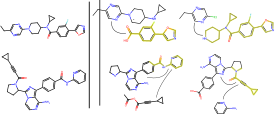
\includegraphics[width=\columnwidth]{fig/inpainting}};

    \begin{scope}[x={(image.south east)},y={(image.north west)}]
      \node[label] at (.16,1.02) {\textbf{Product}};

    \node[label] at (.70,1.02) {\textbf{Generate one reactant conditional on another}};

    \node[label] at (.70,0.56) {\textbf{Generate conditional on desired substructure}};

    \end{scope}
      
  \end{tikzpicture}

\end{document}